% !TEX program = xelatex
\documentclass[a4paper]{article}
\usepackage{amsmath}
\usepackage{amsthm}
\usepackage[left=1.8cm,right=1.8cm,top=2.2cm,bottom=2.0cm]{geometry}
\usepackage{ctex}
\usepackage{enumerate}
\usepackage{fancyhdr}
\usepackage{xpatch}
\usepackage{graphicx} 
\usepackage{float} 
\usepackage{subfigure} 
\usepackage{amsfonts}
\usepackage{mathtools}
\usepackage{framed}
\usepackage{multicol}
\usepackage{listings}
\usepackage{hyperref}
\usepackage{tikz}
\usetikzlibrary{automata,positioning}
\theoremstyle{definition}
\newtheorem*{solution*}{\textbf{Solution:}}
\newtheorem*{proof*}{\textbf{Proof:}}
\newtheorem{theorem}{Theorem}[subsection]
\newtheorem{definition}{Definition}[subsection]
\newtheorem{lemma}{Lemma}[subsection]
\makeatletter

\AtBeginDocument{\xpatchcmd{\@thm}{\thm@headpunct{.}}{\thm@headpunct{}}{}{}}
\makeatother

\pagestyle{fancy}
\renewcommand{\baselinestretch}{1.15}

\usepackage{paralist}
\let\itemize\compactitem
\let\enditemize\endcompactitem
\let\enumerate\compactenum
\let\endenumerate\endcompactenum
\let\description\compactdesc
\let\enddescription\endcompactdesc

% shorten footnote rule
\xpatchcmd\footnoterule
  {.4\columnwidth}
  {1in}
  {}{\fail}

\title{CS 131 Compilers: Discussion 7: Syntax Directed Translation \& Mid Term Preparation1}
\author{\textbf{杨易为}~~\textbf{季杨彪}~~\textbf{尤存翰} \\ \texttt{ \{yangyw,jiyb,youch\}@shanghaitech.edu.cn}}


\begin{document}
\maketitle
\section{Syntax Directed Translation}
Syntax-directed translation refers to a method of compiler implementation where the source language translation is completely driven by the parser. In other words, the parsing process and parse trees are used to direct semantic analysis and the translation of the source program. This can be a separate phase of a compiler or we can augment our conventional grammar with information to control the semantic analysis and translation. Such grammars are called attribute grammars.

We augment a grammar by associating attributes with each grammar symbol that describes its properties. An attribute has a name and an associated value: a string, a number, a type, a memory location, an assigned register—whatever information we need. For example, variables may have an attribute "type" (which records the declared type of a variable, useful later in type-checking) or an integer constant may have an attribute "value" (which we will later need to generate code).

With each production in a grammar, we give semantic rules or actions, which describe how to compute the attribute values associated with each grammar symbol in a production. The attribute value for a parse node may depend on information from its children nodes below or its siblings and parent node above.

Consider this production, augmented with a set of actions that use the "value" attribute for a digit node to store the appropriate numeric value. Below, we use the syntax X.a to refer to the attribute a associated with symbol X.

\begin{center}
  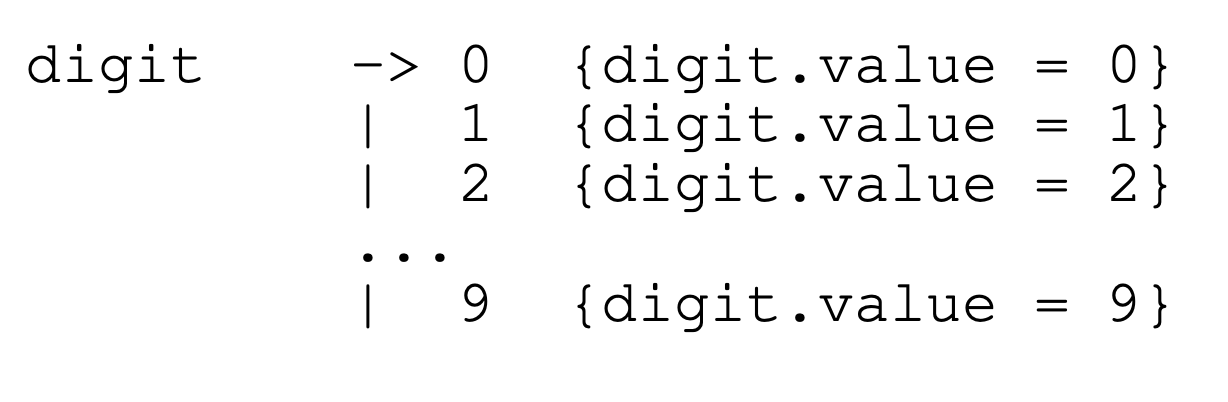
\includegraphics[height=3cm]{img/Snipaste_2021-04-12_17-41-51.png}
  \end{center}
  Attributes may be passed up a parse tree to be used by other productions:
  
  \begin{center}
    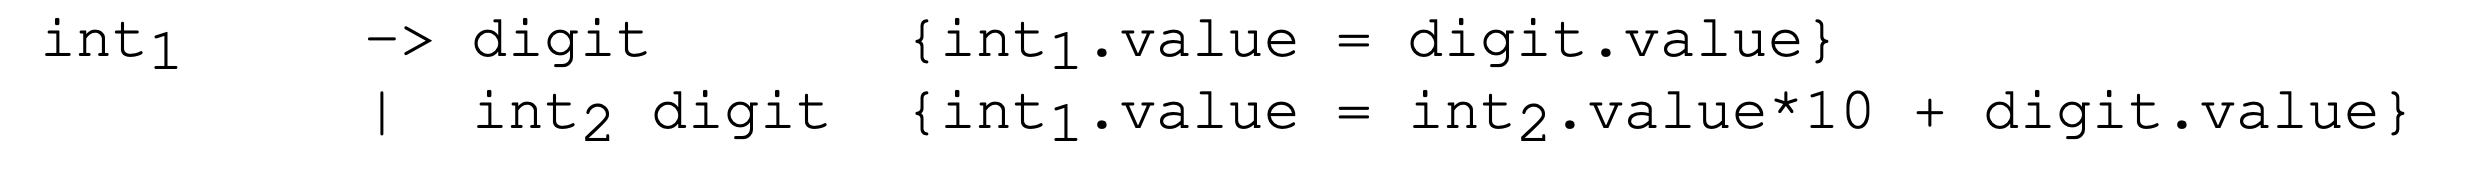
\includegraphics[height=1.2cm]{img/Snipaste_2021-04-12_17-42-34.png}
    \end{center}
    
    There are two types of attributes we might encounter: synthesized or inherited. Synthesized attributes are those attributes that are passed up a parse tree, i.e., the left-
    side attribute is computed from the right-side attributes. The lexical analyzer usually supplies the attributes of terminals and the synthesized ones are built up for the nonterminals and passed up the tree.
    
    \begin{center}
      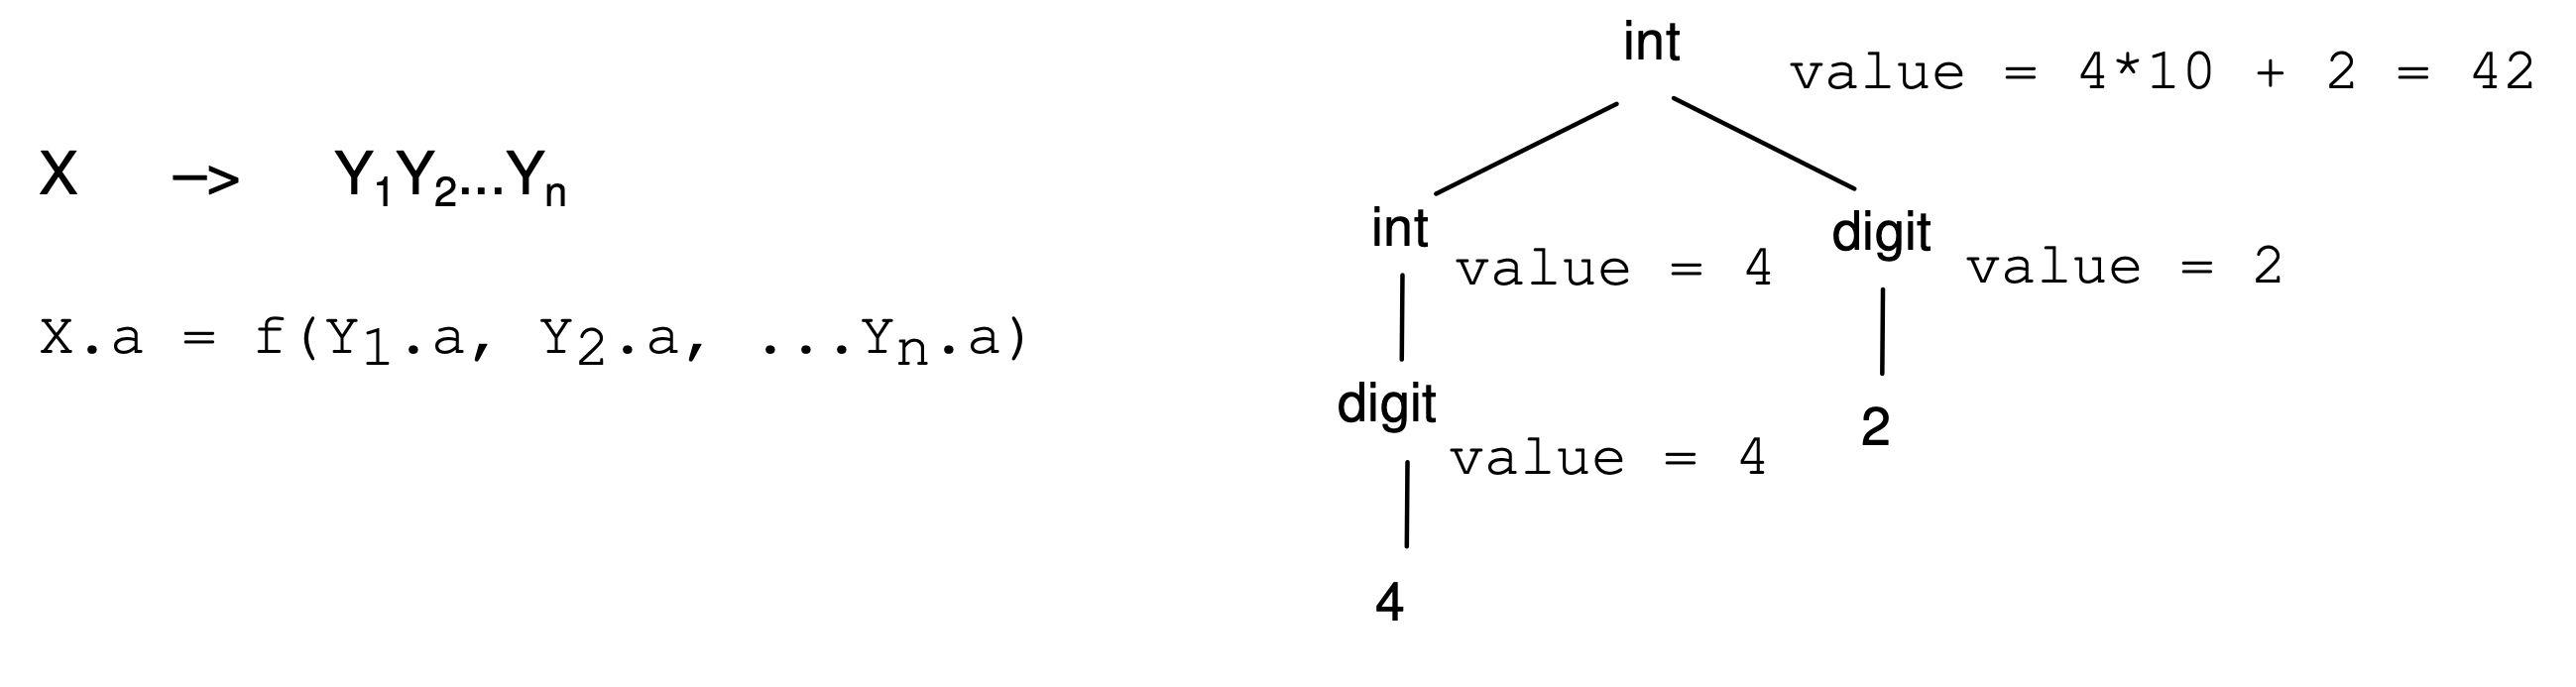
\includegraphics[height=3cm]{img/Snipaste_2021-04-12_17-43-29.png}
      \end{center}
      
      Inherited attributes are those that are passed down a parse tree, i.e., the right-side attributes are derived from the left-side attributes (or other right-side attributes). These attributes are used for passing information about the context to nodes further down the tree.
      \begin{center}
        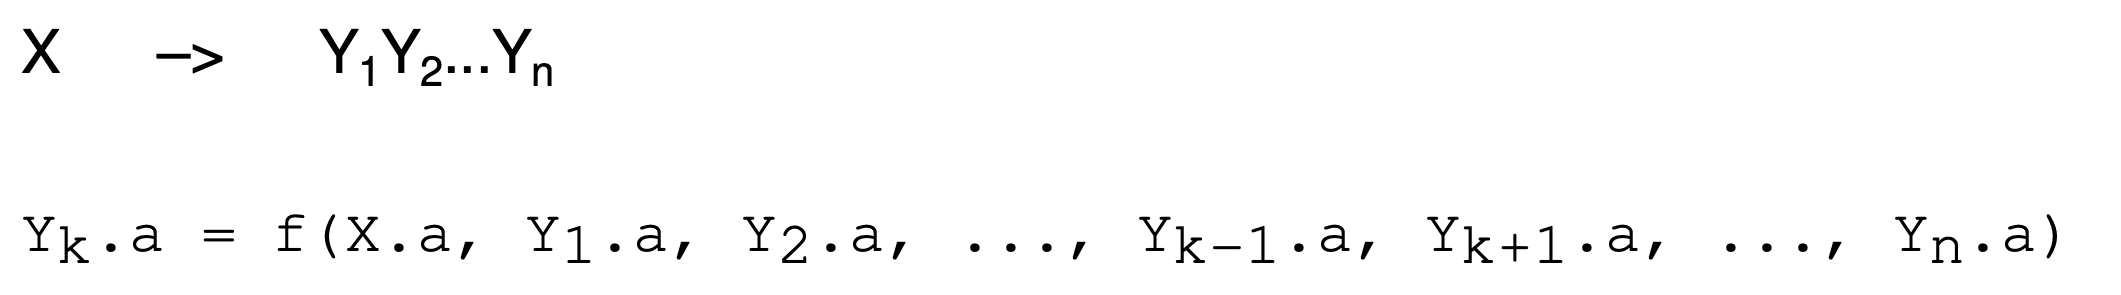
\includegraphics[height=1.5cm]{img/Snipaste_2021-04-12_17-44-09.png}
        \end{center}
Bison is a little bit different, which is bigger than LALR(k).


\section{Mid Term preparation}
\subsection{Regular Expressions}
\begin{enumerate}
   \item Write a regex that matches binary strings divisible by 8.
   \item Provide aregulargrammar for the regex from part (a).
 \end{enumerate}

  \subsection{Finite State Automata}
  \begin{enumerate}
    \item Write the corresponding NFA for the regular expression $(0|1)?(10|01)+$;
    \item Convert the NFA from part (a) into a DFA.
  \end{enumerate}
  
  \subsection{Grammar Rewriting and LL(k) Parsing}
  $$
\begin{aligned}
&\begin{aligned}
S &: E \dashv \\
E: & E+E \\
& \mid E * E
\end{aligned}\\
&\quad 
 \ \mid \text { ID }
\end{aligned}
$$
  \begin{enumerate}
    \item Show that the grammar is ambiguous with two different leftmost derivations of the string $a+b*c$;
    \item Rewrite this grammar so that it preserves the standard order of operations, is LL(1),and is unambiguous.  Draw the resulting tree for the string $a+b*c$;
    \item Write down the equivalent unambiguous grammar that enforces both left associativity and correct precedence.  Why can’t this be achieved with an LL(1) grammar?
  \end{enumerate}

  \subsection{Earley’s Algorithm}

  \begin{center}
    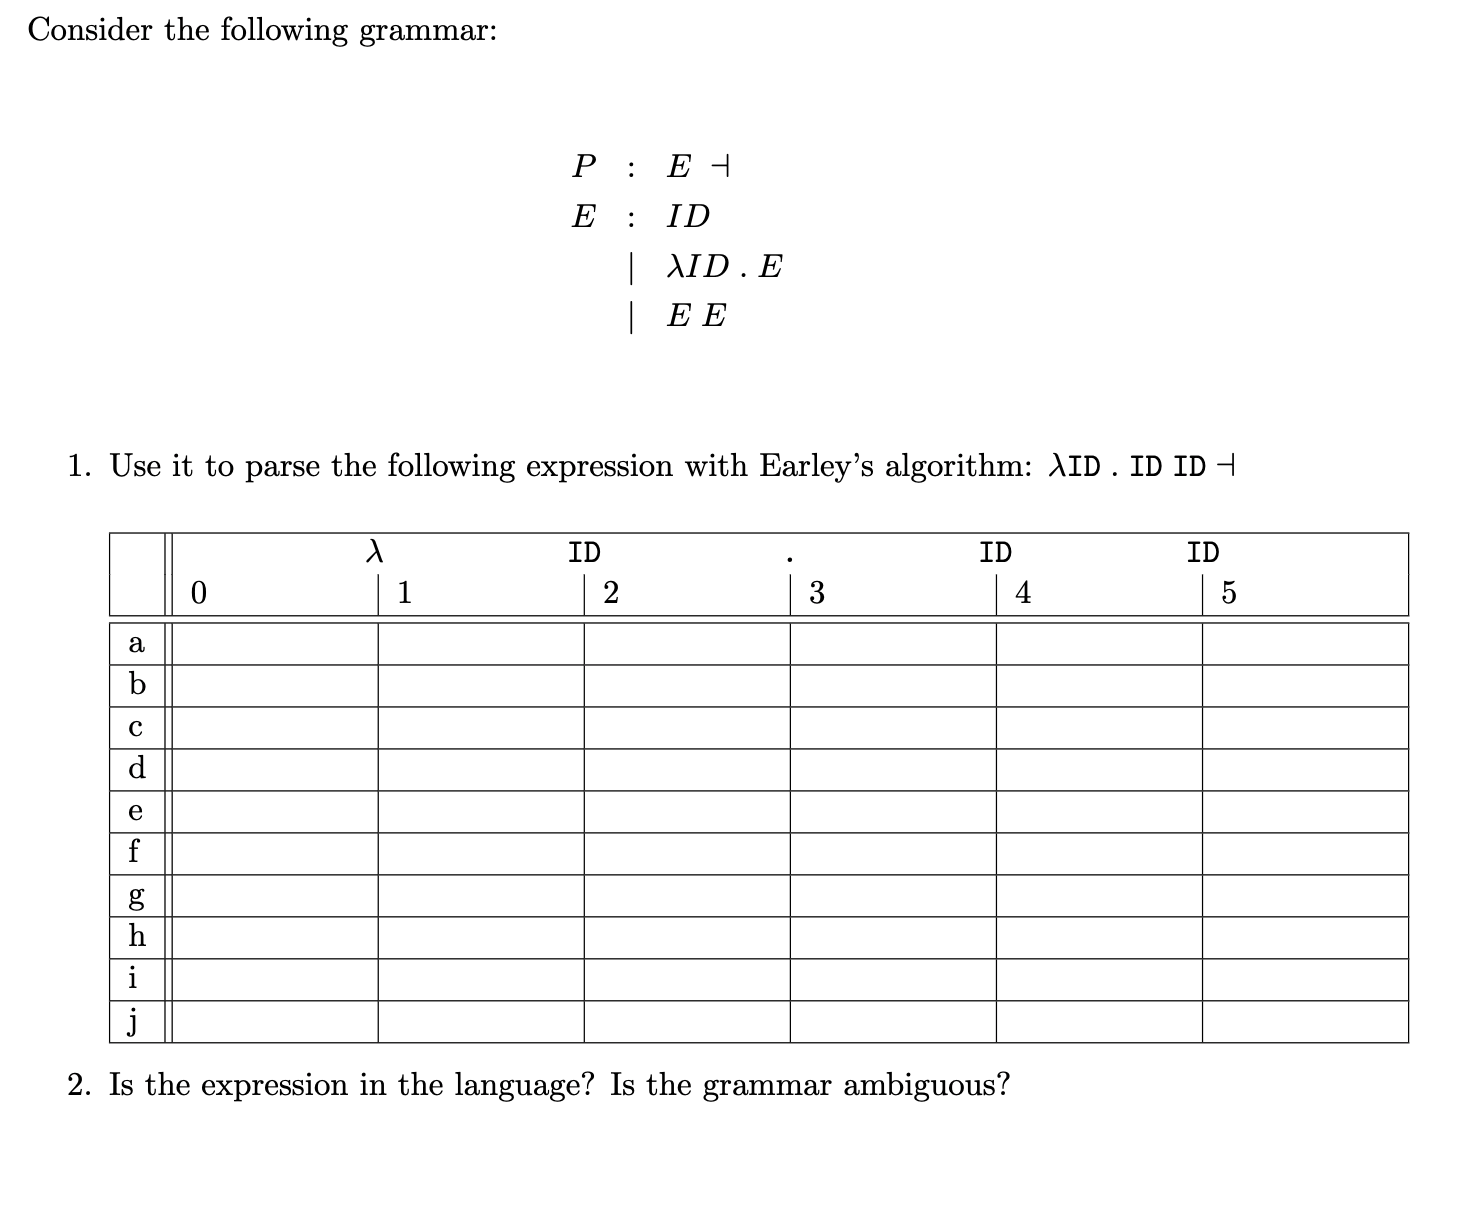
\includegraphics[height=12cm]{img/Snipaste_2021-04-12_17-39-39.png}
    \end{center}
    
\end{document}
